\section{Résultats}
\label{chap:resultats}
% [Votre texte ici]
%\lipsum[1-2]

\subsection{Partie 1}
\label{sec:resultats_partie1}
% [Votre texte ici]
%\lipsum[3]
% Voici un exemple de graphique généré avec le paquet PGFPlots.
% C'est très utile pour les graphiques de performance ou les visualisations de données.
\begin{figure}[H]
    \centering
    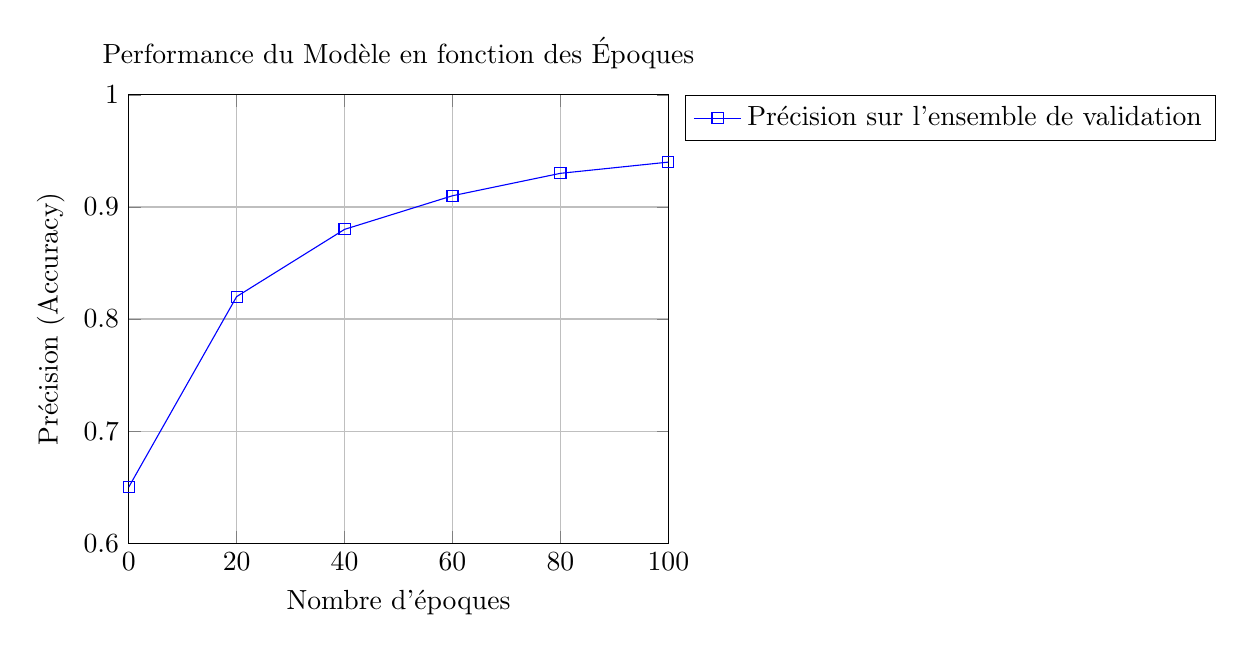
\begin{tikzpicture}
        \begin{axis}[
            title={Performance du Modèle en fonction des Époques},
            xlabel={Nombre d'époques},
            ylabel={Précision (Accuracy)},
            xmin=0, xmax=100,
            ymin=0.6, ymax=1,
            xtick={0,20,40,60,80,100},
            ytick={0.6,0.7,0.8,0.9,1.0},
            legend pos=outer north east,
            grid=major,
            ]
            \addplot[color=blue, mark=square,]
            coordinates {
                (0,0.65)(20,0.82)(40,0.88)(60,0.91)(80,0.93)(100,0.94)
            };
            \addlegendentry{Précision sur l'ensemble de validation}
        \end{axis}
    \end{tikzpicture}
    \caption{Courbe d'apprentissage du modèle d'IA.}
    \label{fig:learning_curve}
\end{figure}

\subsubsection{Sous-partie 1}
\label{ssec:resultats_p1_s1}
% [Votre texte ici]
%\lipsum[4]

\subsubsection{Sous-partie 2}
\label{ssec:resultats_p1_s2}
% [Votre texte ici]
%\lipsum[5]

\subsubsection{Sous-partie 3}
\label{ssec:resultats_p1_s3}
% [Votre texte ici]
%\lipsum[6]

\subsection{Partie 2}
\label{sec:resultats_partie2}
% [Votre texte ici]
%\lipsum[7]
% Voici un autre exemple d'image, cette fois pour montrer un résultat final.
% La taille est ici fixée à 50% de la largeur du texte.
\begin{figure}[H]
    \centering
    \includegraphics[width=0.5\linewidth]{figs/rendu.png}
    \caption{Exemple de rendu visuel généré par la solution.}
    \label{fig:rendu_final}
\end{figure} 